\documentclass[onlymath]{beamer}

%%%%%%%%%%%%%%%%%%%%%%%%%%%%%%%%%%%%%%%%%%%%%%%%%%%%%%%%%%%%%%%%%%%%%
% COLORES
%%%%%%%%%%%%%%%%%%%%%%%%%%%%%%%%%%%%%%%%%%%%%%%%%%%%%%%%%%%%%%%%%%%%%
\usepackage{color}

\definecolor{titulo}{HTML}{750202}

\definecolor{seccion}{HTML}{360101}
\definecolor{sombra_seccion}{HTML}{750202}

\definecolor{subseccion}{HTML}{750202}
\definecolor{sombra_subseccion}{HTML}{A75E5E}

\definecolor{listas}{HTML}{750202}

\definecolor{tb-std}{HTML}{360101}
\definecolor{tb-ale}{HTML}{02020A}
\definecolor{tb-exa}{HTML}{02020A}
\definecolor{fb-std}{HTML}{A75E5E}
\definecolor{fb-ale}{HTML}{d01800}
\definecolor{fb-exa}{HTML}{fee8ef}
\definecolor{cb-std}{HTML}{fee8ef}
\definecolor{cb-ale}{HTML}{fee8ef}
\definecolor{cb-exa}{HTML}{fff2f2}

\definecolor{primero}{HTML}{fee8ef}
\definecolor{segundo}{HTML}{ffe8ef}
\definecolor{tercero}{HTML}{ffe8ee}
\definecolor{cuarto}{HTML}{ffecf1}
\definecolor{quinto}{HTML}{fff0f4}

%%%%%%%%%%%%%%%%%%%%%%%%%%%%%%%%%%%%%%%%%%%%%%%%%%%%%%%%%%%%%%%%%%%%%
% TEMA
%%%%%%%%%%%%%%%%%%%%%%%%%%%%%%%%%%%%%%%%%%%%%%%%%%%%%%%%%%%%%%%%%%%%%
\useinnertheme{circles} % Tipo de tema para el índice
\setbeamertemplate{itemize items}[triangle]
\setbeamertemplate{enumerate items}[default]
\setbeamerfont{title}{size = \huge}
\setbeamerfont{frametitle}{size = \bfseries\Large}
\setbeamercolor{normal text}{fg = black} % Color del texto
\setbeamercolor{frametitle}{fg = titulo} % Color del título de las diapositivas
\setbeamercolor{title}{fg = titulo} % Color del título de la presentación
\setbeamercolor{section in toc}{fg = seccion} % Color de la sección actual
\setbeamercolor{section in toc shaded}{fg = sombra_seccion} % Color de la sección sombreada
\setbeamercolor{subsection in toc}{fg = subseccion} % Color de la subsección actual
\setbeamercolor{subsection in toc shaded}{fg = sombra_subseccion} % Color de la subsección sombreada
\setbeamercolor{item}{fg = listas} % Color de los ítems
\setbeamercolor{subitem}{fg = listas} % Color de los subítems
\setbeamercolor{subsubitem}{fg = listas} % Color de los subsubítems
\setbeamercolor{description item}{fg = listas} % Color del título de los ítems en las descripciones
\setbeamercolor{caption}{fg = black} % Color de las etiquetas
\setbeamercolor{caption name}{fg = black} % Color de las etiquetas
% Bloque estándar
\setbeamercolor{block title}{fg = tb-std, bg = fb-std} % Título del bloque
\setbeamercolor{block body}{bg = cb-std} % Cuerpo del bloque
% Bloque Alert
\setbeamercolor{block title alerted}{fg = tb-ale, bg = fb-ale} % Título del bloque
\setbeamercolor{block body alerted}{bg = cb-ale} % Cuerpo del bloque
% Bloque Example
\setbeamercolor{block title example}{fg = tb-exa, bg = fb-exa} % Título del bloque
\setbeamercolor{block body example}{bg = cb-exa} % Cuerpo del bloque

%%%%%%%%%%%%%%%%%%%%%%%%%%%%%%%%%%%%%%%%%%%%%%%%%%%%%%%%%%%%%%%%%%%%%
% MISCELÁNEO
%%%%%%%%%%%%%%%%%%%%%%%%%%%%%%%%%%%%%%%%%%%%%%%%%%%%%%%%%%%%%%%%%%%%%
\beamertemplatenavigationsymbolsempty % Elimina la barra de navegación
\usepackage[T1]{fontenc}
\usepackage[sfdefault]{AlegreyaSans} %% Option 'black' gives heavier bold face
%% The 'sfdefault' option to make the base font sans serif
\renewcommand*\oldstylenums[1]{{\AlegreyaSansOsF #1}}
\usepackage{babel}
\usepackage{graphicx} % Insertar imágenes


%%%%%%%%%%%%%%%%%%%%%%%%%%%%%%%%%%%%%%%%%%%%%%%%%%%%%%%%%%%%%%%%%%%%%
% PORTADA
%%%%%%%%%%%%%%%%%%%%%%%%%%%%%%%%%%%%%%%%%%%%%%%%%%%%%%%%%%%%%%%%%%%%%
\title{\fontsize{50pt}{50pt}{\textbf{Workout App}}}
\subtitle{\LARGE{Design}}
\author{\textit{Web Platform Developement 2}}
\date{Manuel Gachs Ballegeer}

%%%%%%%%%%%%%%%%%%%%%%%%%%%%%%%%%%%%%%%%%%%%%%%%%%%%%%%%%%%%%%%%%%%%%
% DOCUMENTO
%%%%%%%%%%%%%%%%%%%%%%%%%%%%%%%%%%%%%%%%%%%%%%%%%%%%%%%%%%%%%%%%%%%%%

\usepackage{graphicx}
\begin{document}
\frame{
	\maketitle
}
\frame{
	\frametitle{Index}
	\tableofcontents
}
\section{Functionality \& Software}
\frame{
	\frametitle{Functionality \& Software}
	The app will be developed in Node.js using the \textbf{Express}
	framewok. For database management, \textbf{NeDB} will be used, and 
	html templates will used via \textbf{Mustache}.
	\smallskip
	\begin{columns}[t]
	\begin{column}{.5\textwidth}
	\textbf{Required:}
	\begin{itemize}
		\item Add training goals (any week)$^*$.
		\item Delete training goals (any week).
		\item Modify training goals (any week).
		\item Record training achievements (current week).
		\item See the incomplete training goals of the week.
		\item Share a training plan.
		\item Login.
	\end{itemize}
	\end{column}
	\begin{column}{.5\textwidth}
	\textbf{Extra:}
	\begin{itemize}
		\item Sign up.
		\item Select a preset plan for a week.
		\item See the weekly progress of an exercise.
		\item See the records on all exercises.
		\item See the training plan of any week.
	\end{itemize}
	\end{column}
	\end{columns}
	\bigskip
	$^*$\footnotesize{Training goals are selected from a list.}
}
\section{Wireframes}
\subsection{Landing page}
\frame{
	\frametitle{Wireframes. Landing page}
	\begin{figure}
		
\includegraphics[scale=0.3]{images/1homepage.png}
		\label{landing_page}
	\end{figure}
}
\subsection{Login \& Sign up}
\frame{
	\frametitle{Wireframes. Login \& Sign up}
	\begin{figure}
		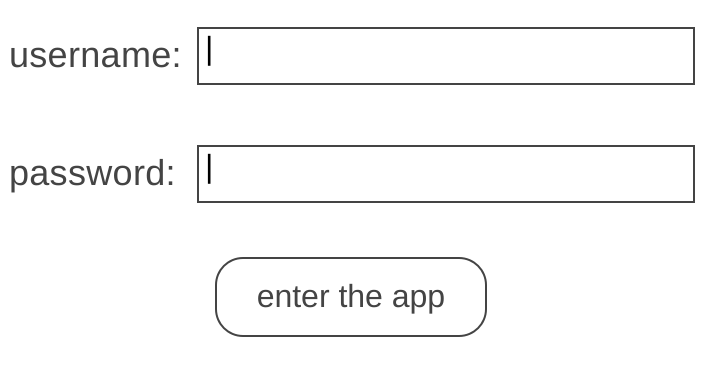
\includegraphics[scale=0.3]{images/2login.png}
		\label{sign_up_login}
	\end{figure}
}
\subsection{Userpage}
\frame{
	\frametitle{Wireframes. Userpage}
	\begin{figure}
		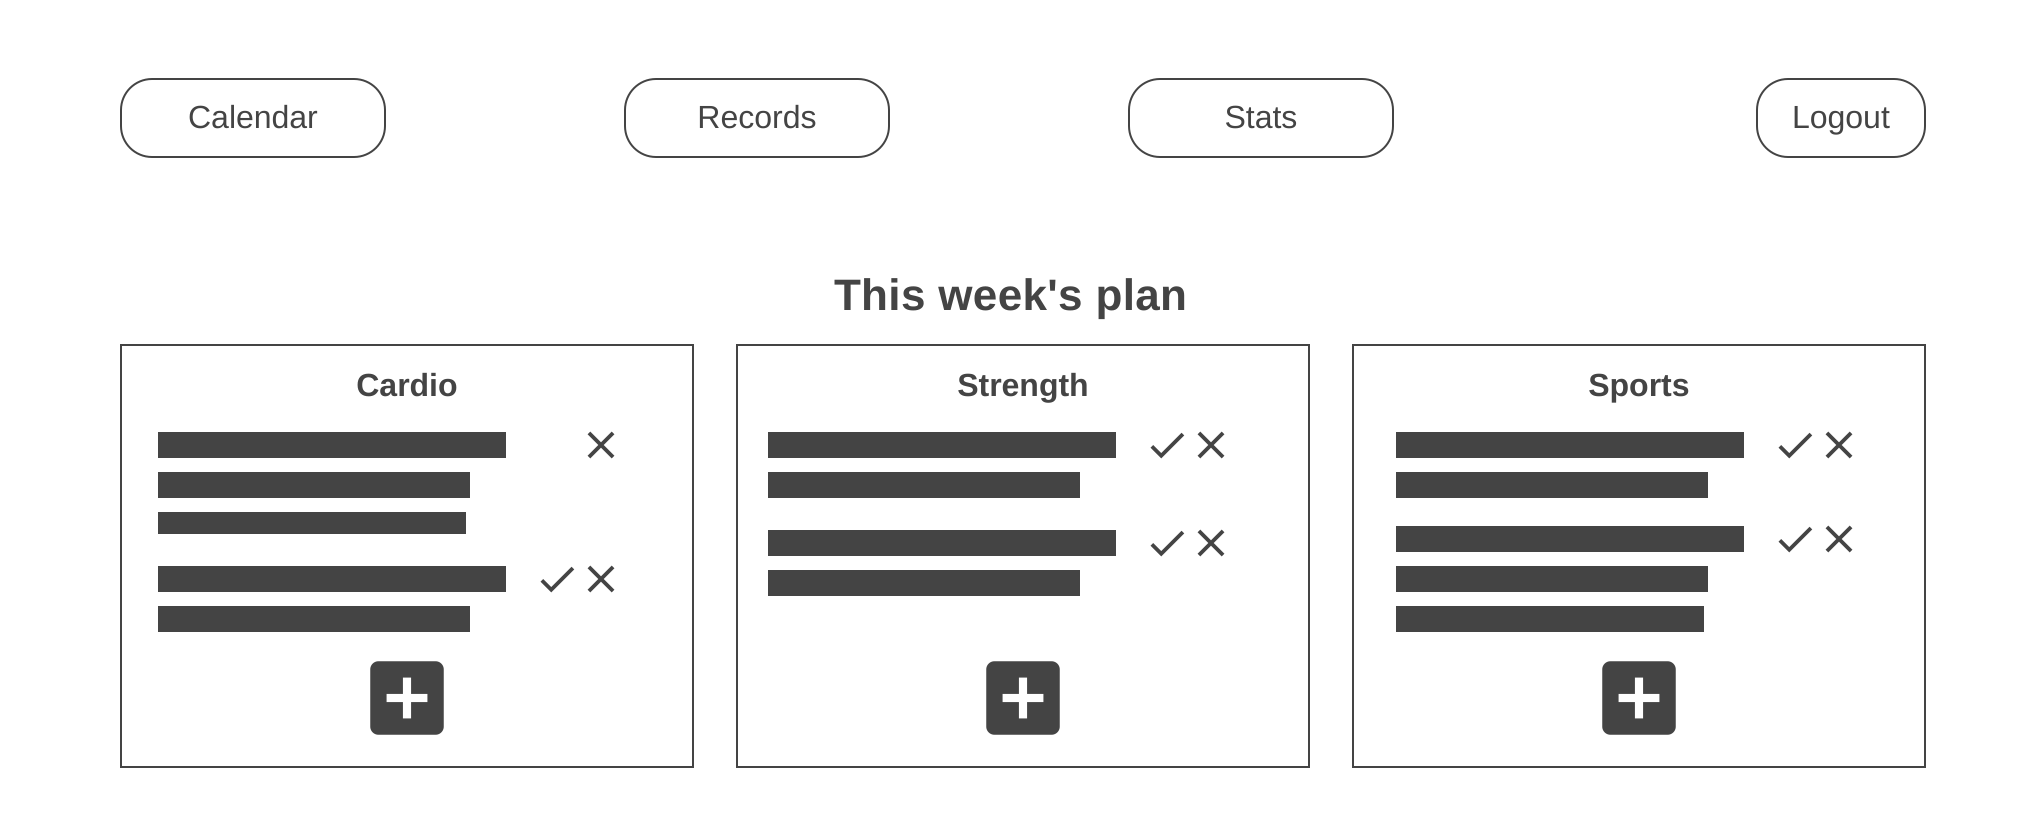
\includegraphics[scale=0.15]{images/3userpage.png}
		\label{userpage}
	\end{figure}
}
\subsection{Calendar}
\frame{
	\frametitle{Wireframes. Calendar}
	Week with an existing training plan.
	\begin{figure}
		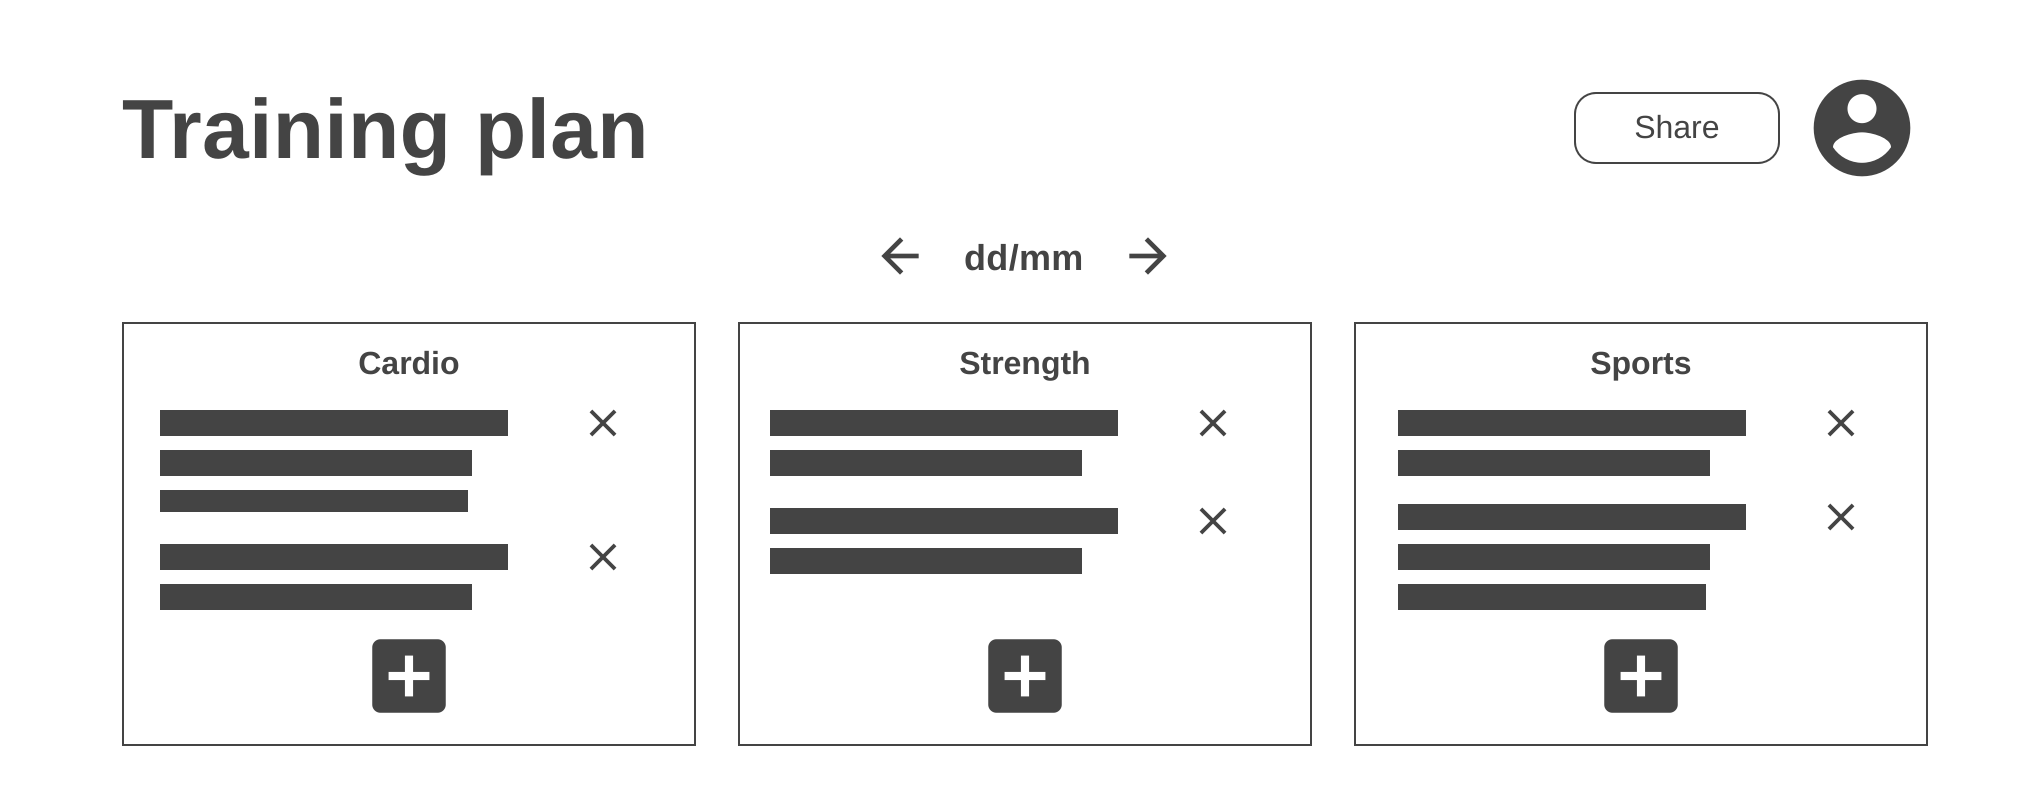
\includegraphics[scale=0.15]{images/4calendar.png}
	\end{figure}
}
\frame{
	Week without a training plan.
	\begin{figure}
		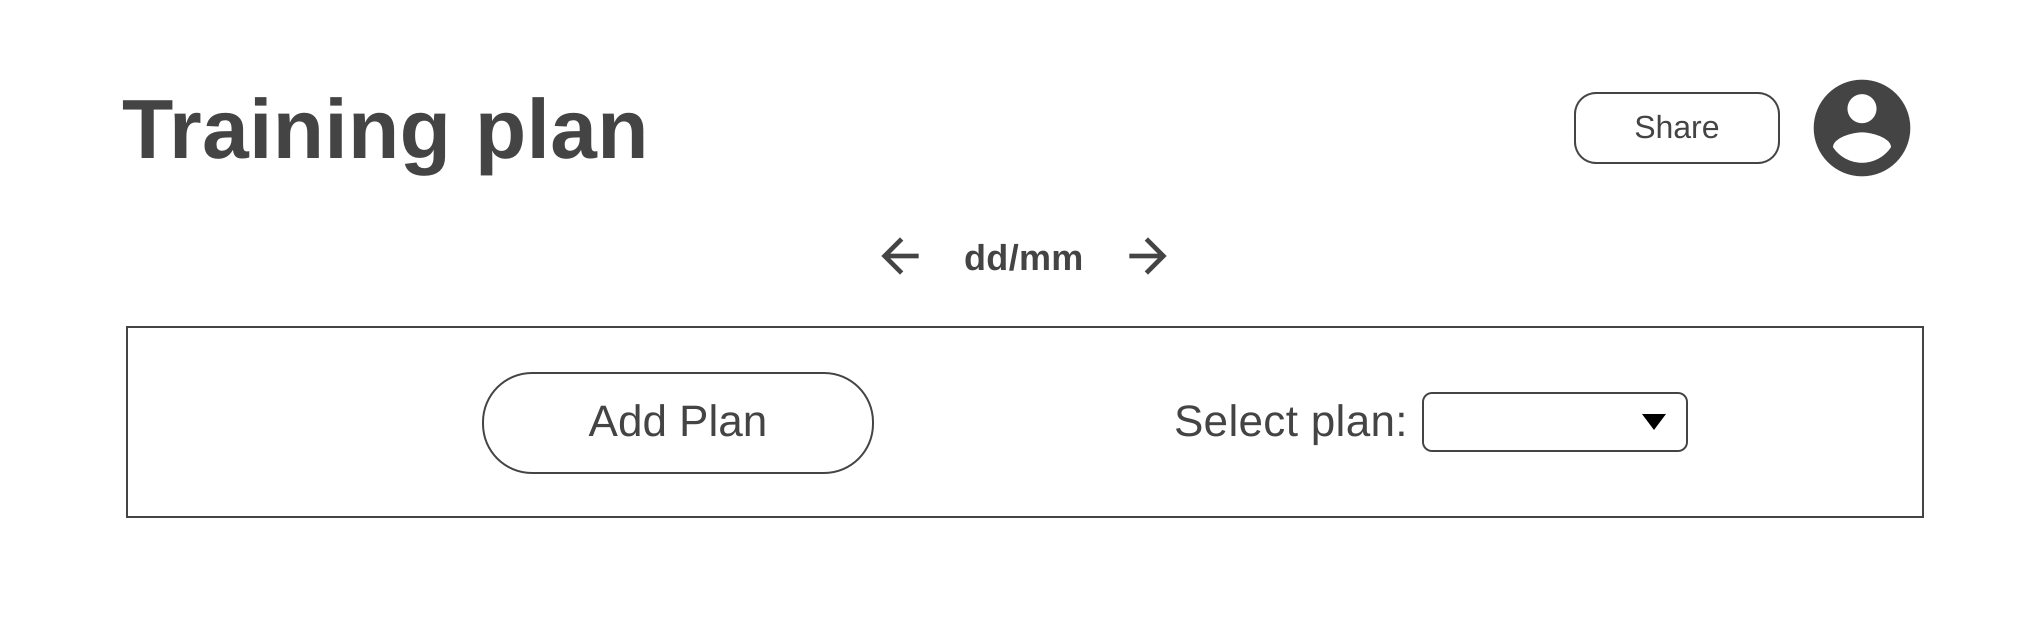
\includegraphics[scale=0.15]{images/5calendarvoid.png}
	\end{figure}
}
\subsection{New exercise}
\frame{
	\frametitle{Wireframes. New exercise}
	\begin{figure}
		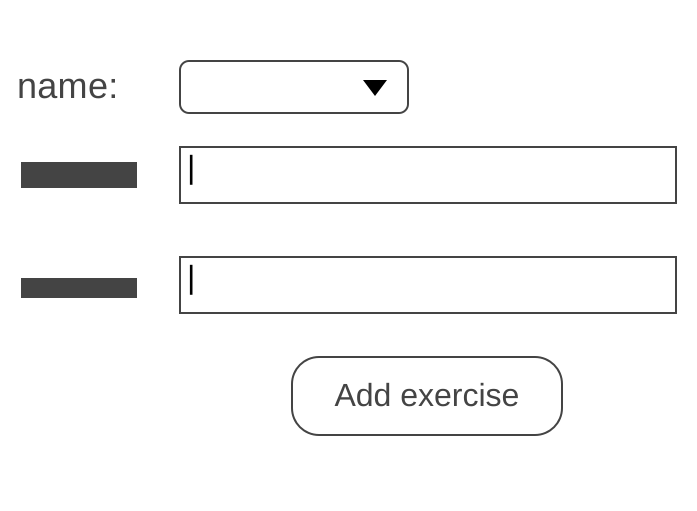
\includegraphics[scale=0.3]{images/6new.png}
	\end{figure}
}
\subsection{Records}
\frame{
	\frametitle{Wireframes. Records}
	\begin{figure}
		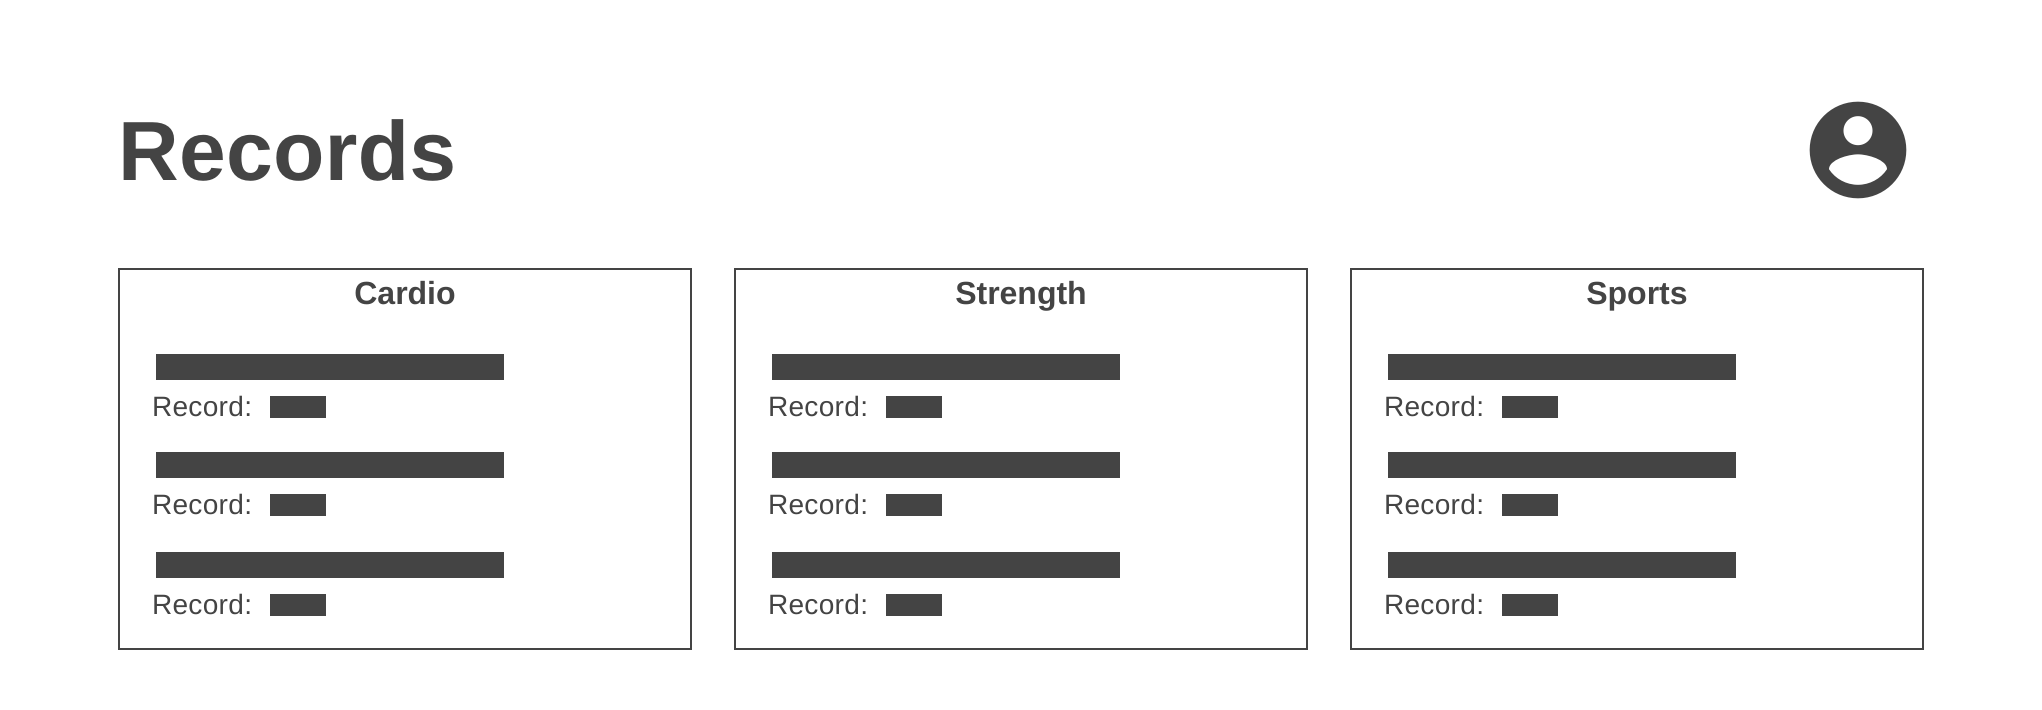
\includegraphics[scale=0.15]{images/7records.png}
	\end{figure}
}
\subsection{Stats}
\frame{
	\frametitle{Wirerames. Stats}
	\begin{figure}
		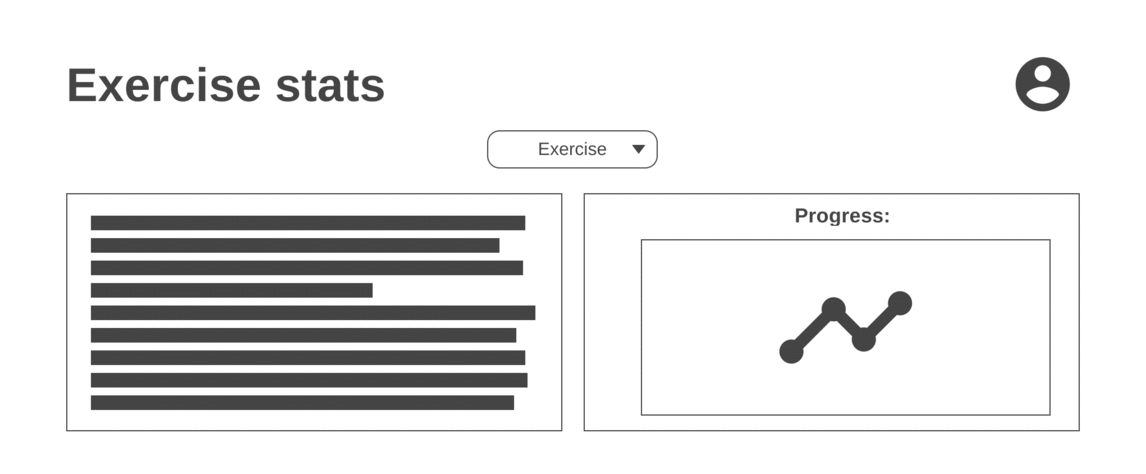
\includegraphics[scale=0.25]{images/8stats.png}
	\end{figure}
}
\section{Use cases}
\subsection{User}
\frame{
	\frametitle{Use cases. User}
	With a regular user as an actor, there are two use cases: Logging in
	and signing up.
	\begin{figure}
		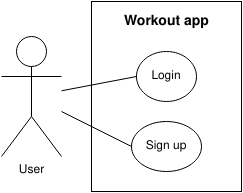
\includegraphics[scale=0.8]{images/user_use_case.png}
	\end{figure}
}
\subsection{Logged user}
\frame{
	\frametitle{Use cases. Logged user}
	As a logged user, there are twelve use cases. They can be divided in
	those that interact with a training plan and those that don't.
	\begin{columns}
		\begin{column}{0.5\textwidth}
			\begin{figure}
				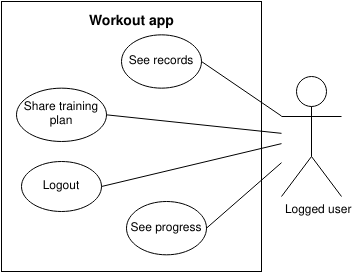
\includegraphics[scale=0.4]{images/logged_user_use_case_1.png}
			\end{figure}
		\end{column}
		\begin{column}{0.5\textwidth}
			\begin{figure}
				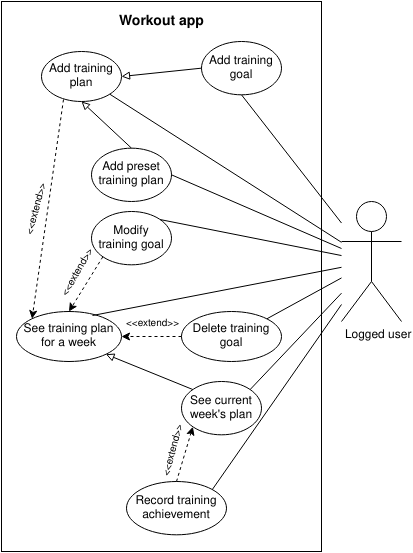
\includegraphics[scale=0.35]{images/logged_user_use_case_2.png}
			\end{figure}
		\end{column}
	\end{columns}
}
\subsection{Global diagram}
\frame{
	\frametitle{Use cases. Global diagram}
	\begin{figure}
		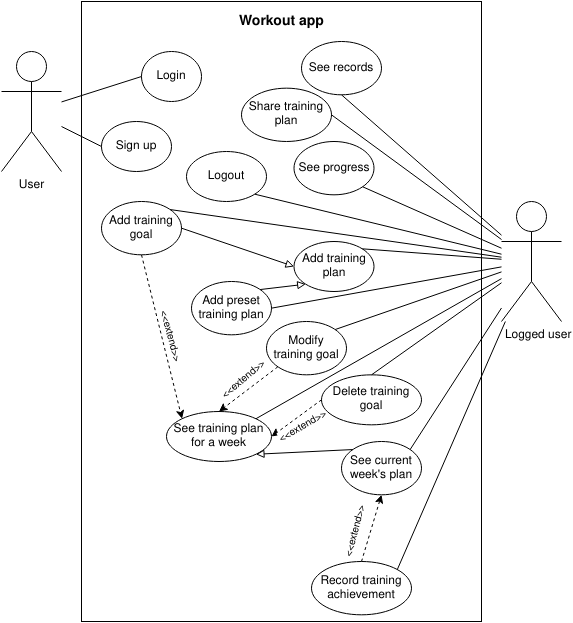
\includegraphics[scale=0.37]{images/use_case.png}
	\end{figure}
}
\section{Class diagram}
\frame{
	\frametitle{Class diagram}
	\begin{figure}
		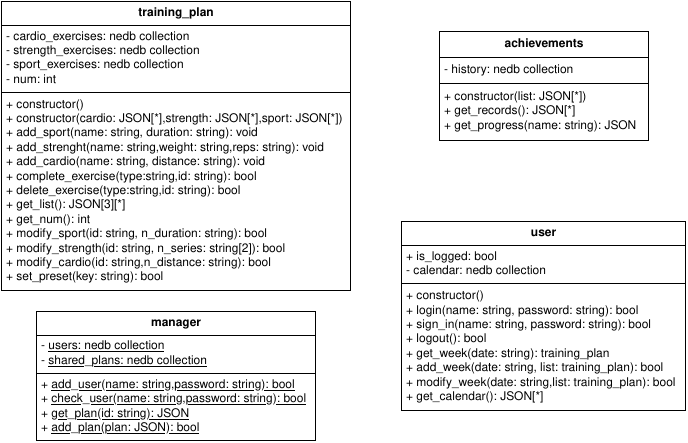
\includegraphics[scale=0.4]{images/classes.png}
	\end{figure}
}
\section{Collections}
\frame{
	\frametitle{Collections}
	\begin{center}
		\textbf{Exercises collections} (\textit{class training\_plan})
	\end{center}
	\begin{figure}
		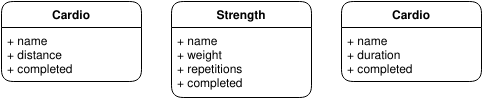
\includegraphics[scale=0.4]{images/training_plan.png}
	\end{figure}
	\begin{columns}
		\begin{column}{0.5\textwidth}
			\begin{center}
				\textbf{Calendar collection}\\(\textit{class user})
			\end{center}
			\begin{figure}
				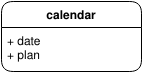
\includegraphics[scale=0.4]{images/user.png}
			\end{figure}
		\end{column}
		\begin{column}{0.5\textwidth}
			\begin{center}
				\textbf{History collection}\\(\textit{class achievements})
			\end{center}
			\begin{figure}
				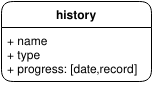
\includegraphics[scale=0.4]{images/achievements.png}
			\end{figure}
		\end{column}
	\end{columns}
	\begin{center}
		\textbf{Management collections} (\textit{class manager})
	\end{center}
	\begin{figure}
		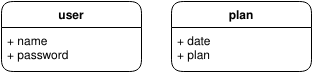
\includegraphics[scale=0.4]{images/manager.png}
	\end{figure}
}
\end{document}